\section{Soil Data Cleaning Summary}\label{annexe:soil-cleaning-summary}

\subsection{Spatial Visualization of Soil Variables}
\begin{figure}[H]
    \centering
    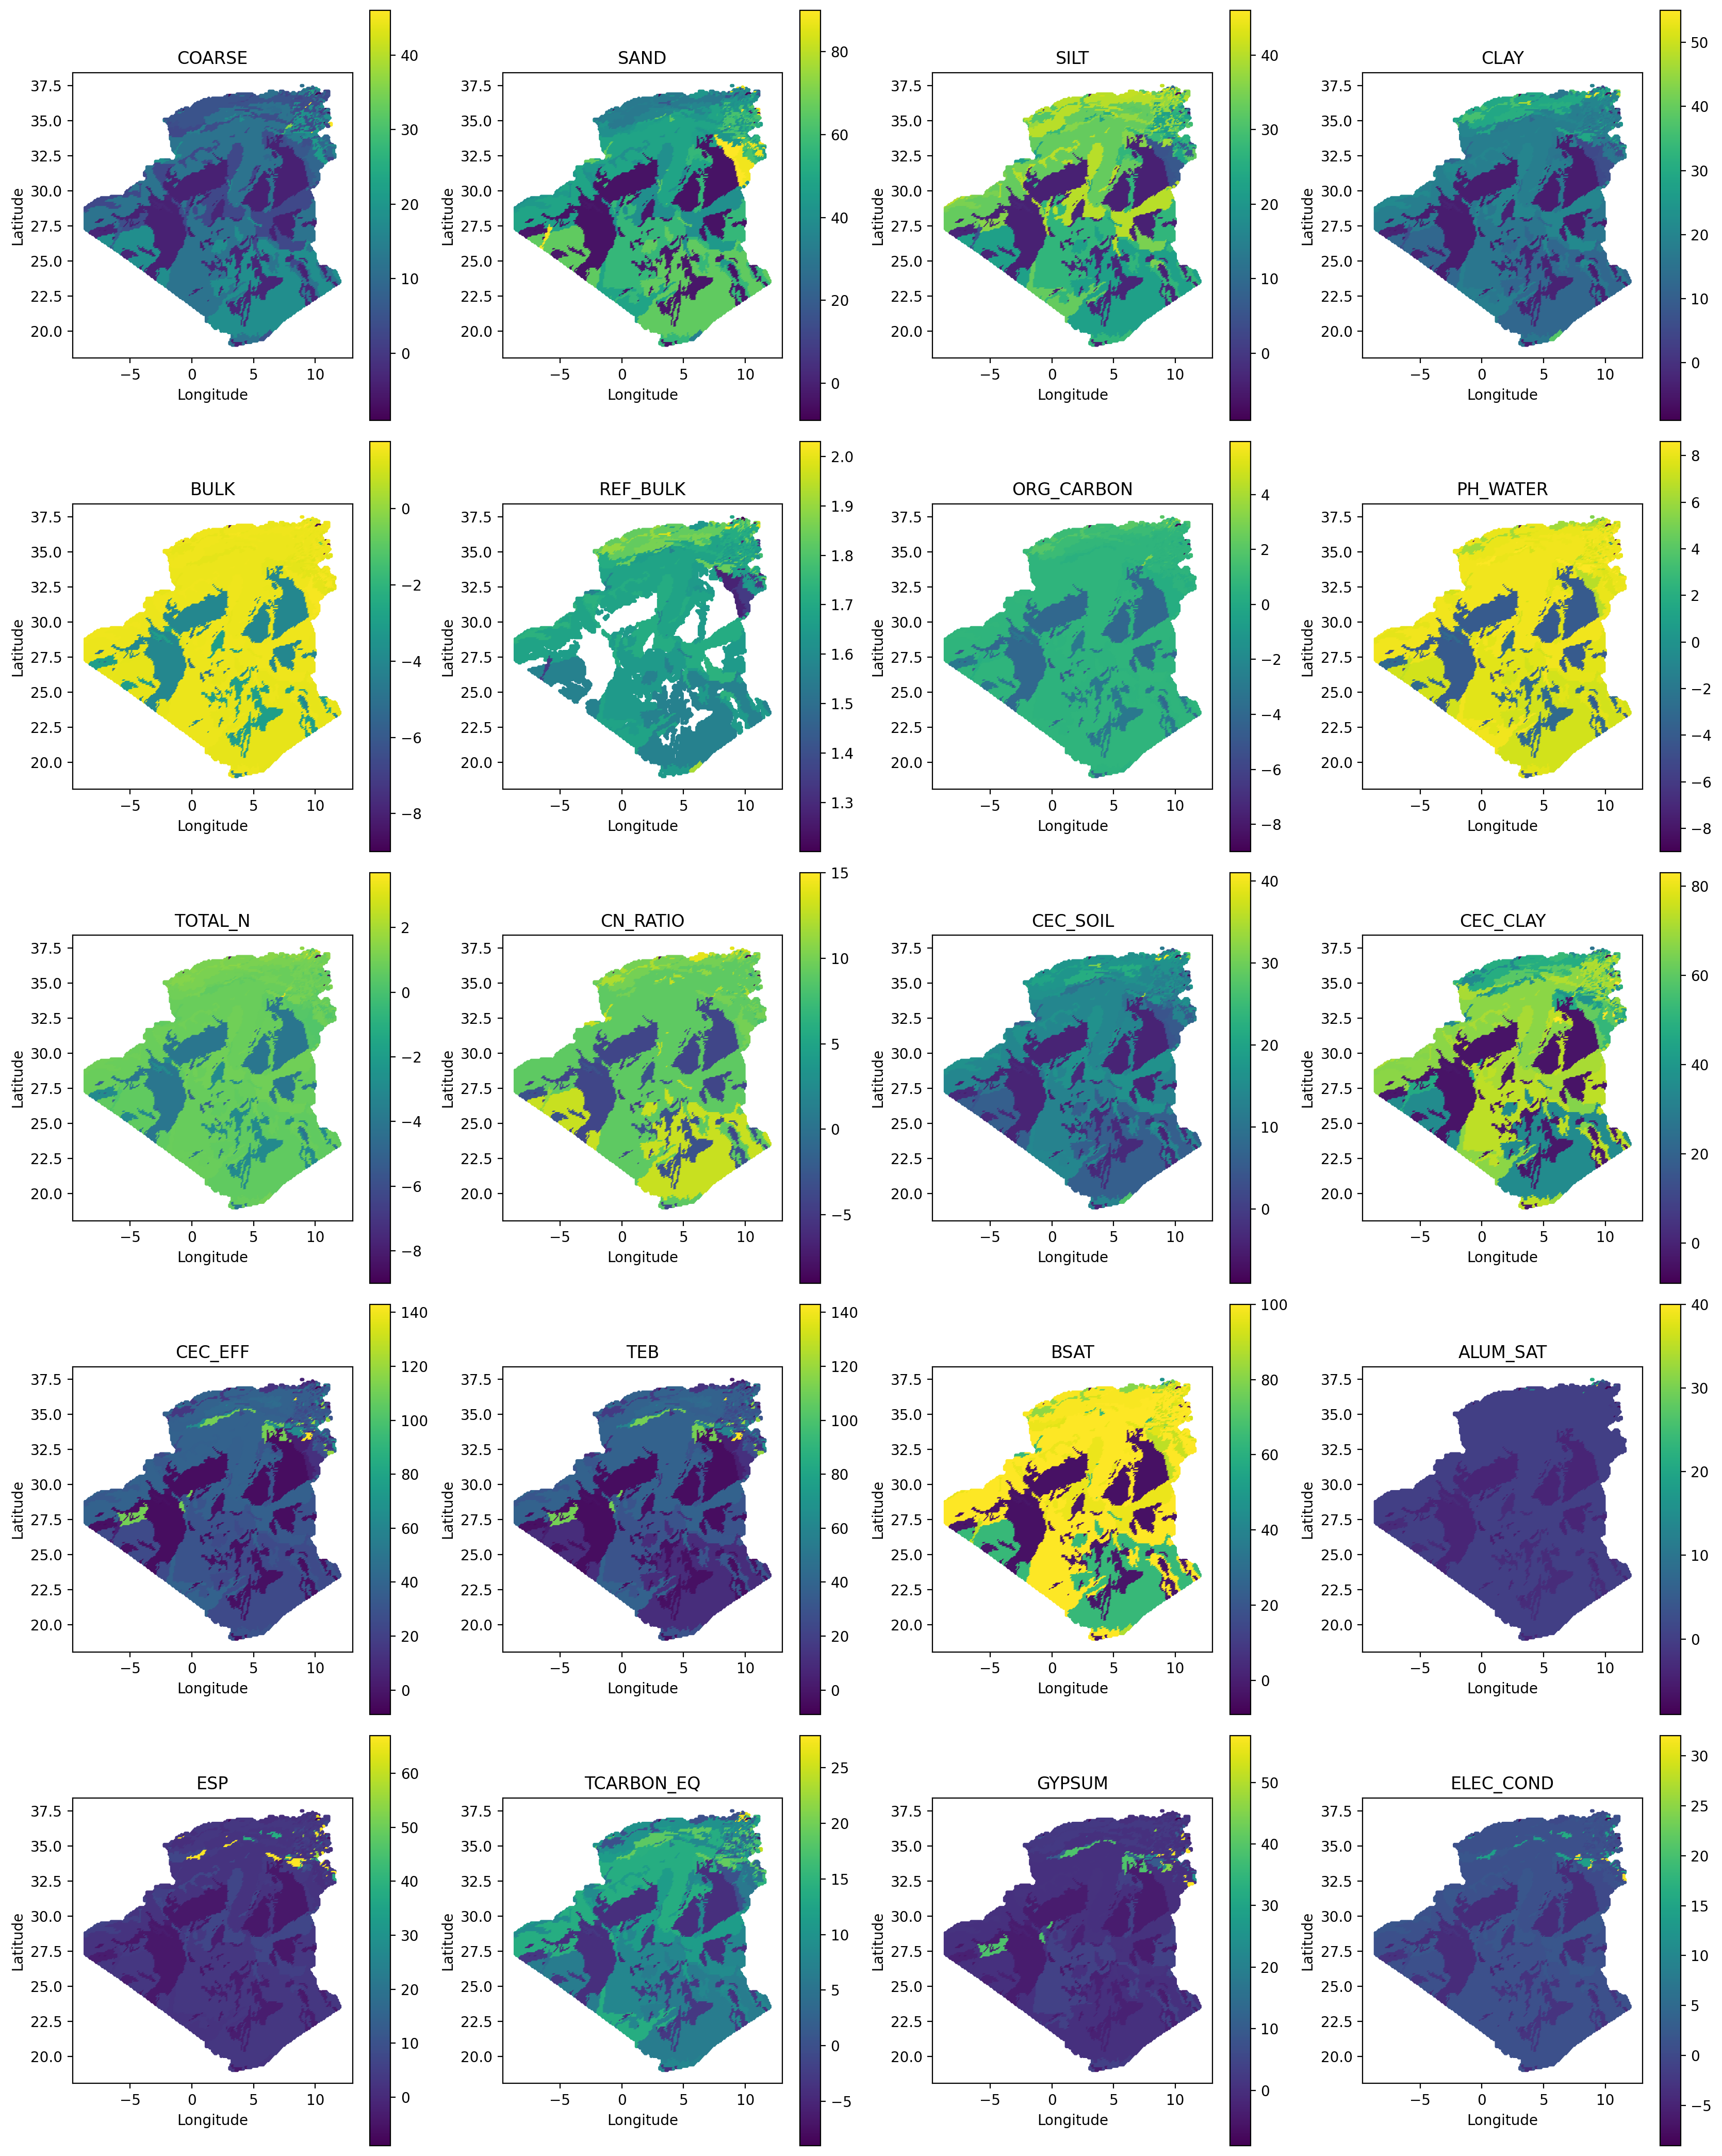
\includegraphics[width=0.65\textwidth]{images/Soil/soil_maps_numeric_variation}
    \caption{Spatial variation maps (subplot grid) of the numeric soil variables over the study area.}\label{fig:soil-maps-numeric}
\end{figure}

\subsection{BallTree Algorithm in the Context of Soil Data}

The BallTree algorithm played a central role in enabling efficient and spatially meaningful imputation. A BallTree recursively partitions the data space into nested hyperspherical regions (``balls''), allowing rapid nearest-neighbor searches compared to brute-force approaches\cite{omohundro1989five, scikit-learn-balltree}. 

In this study, the use of the haversine metric ensured that distances between points were computed as true great-circle distances on the Earth's surface, making the notion of ``nearest'' geographically accurate\cite{haversine}. This was particularly important for soil properties, which are spatially autocorrelated. Without a spatial indexing structure such as BallTree, querying neighbors for 5,480 invalid records against a large geospatial dataset would have been computationally prohibitive. The BallTree approach therefore provided both efficiency and physical relevance.

\begin{figure}[H]
    \centering
    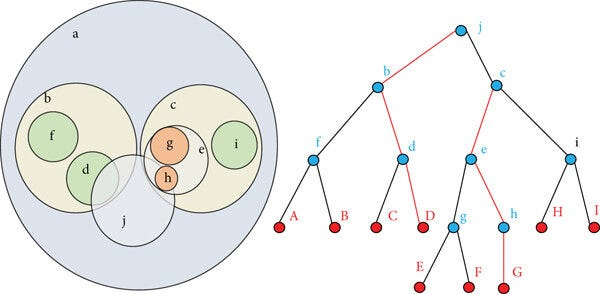
\includegraphics[width=0.7\textwidth]{images/Soil/BallTree.jpg}
    \caption{Conceptual illustration of the BallTree data structure, showing recursive spatial partitioning and efficient nearest-neighbor search.}\label{fig:balltree}
\end{figure}


\subsection{Residual Outliers After Imputation}

After correcting invalid negative records using spatial nearest-neighbor imputation, the soil dataset was re-evaluated for remaining outliers. Although the physically impossible values were successfully eliminated, statistical outliers were still detected across several soil variables. These remaining outliers do not necessarily correspond to data errors, but rather reflect natural soil heterogeneity, extreme environmental conditions, or localized geochemical regimes.

Figure~\ref{fig:soil_kde_after_imputation} and Figure~\ref{fig:soil_qq_after_imputation} summarize the post-imputation distributions using kernel density estimates (KDE) and Quantiles plots, respectively.

\begin{figure}[H]
\centering
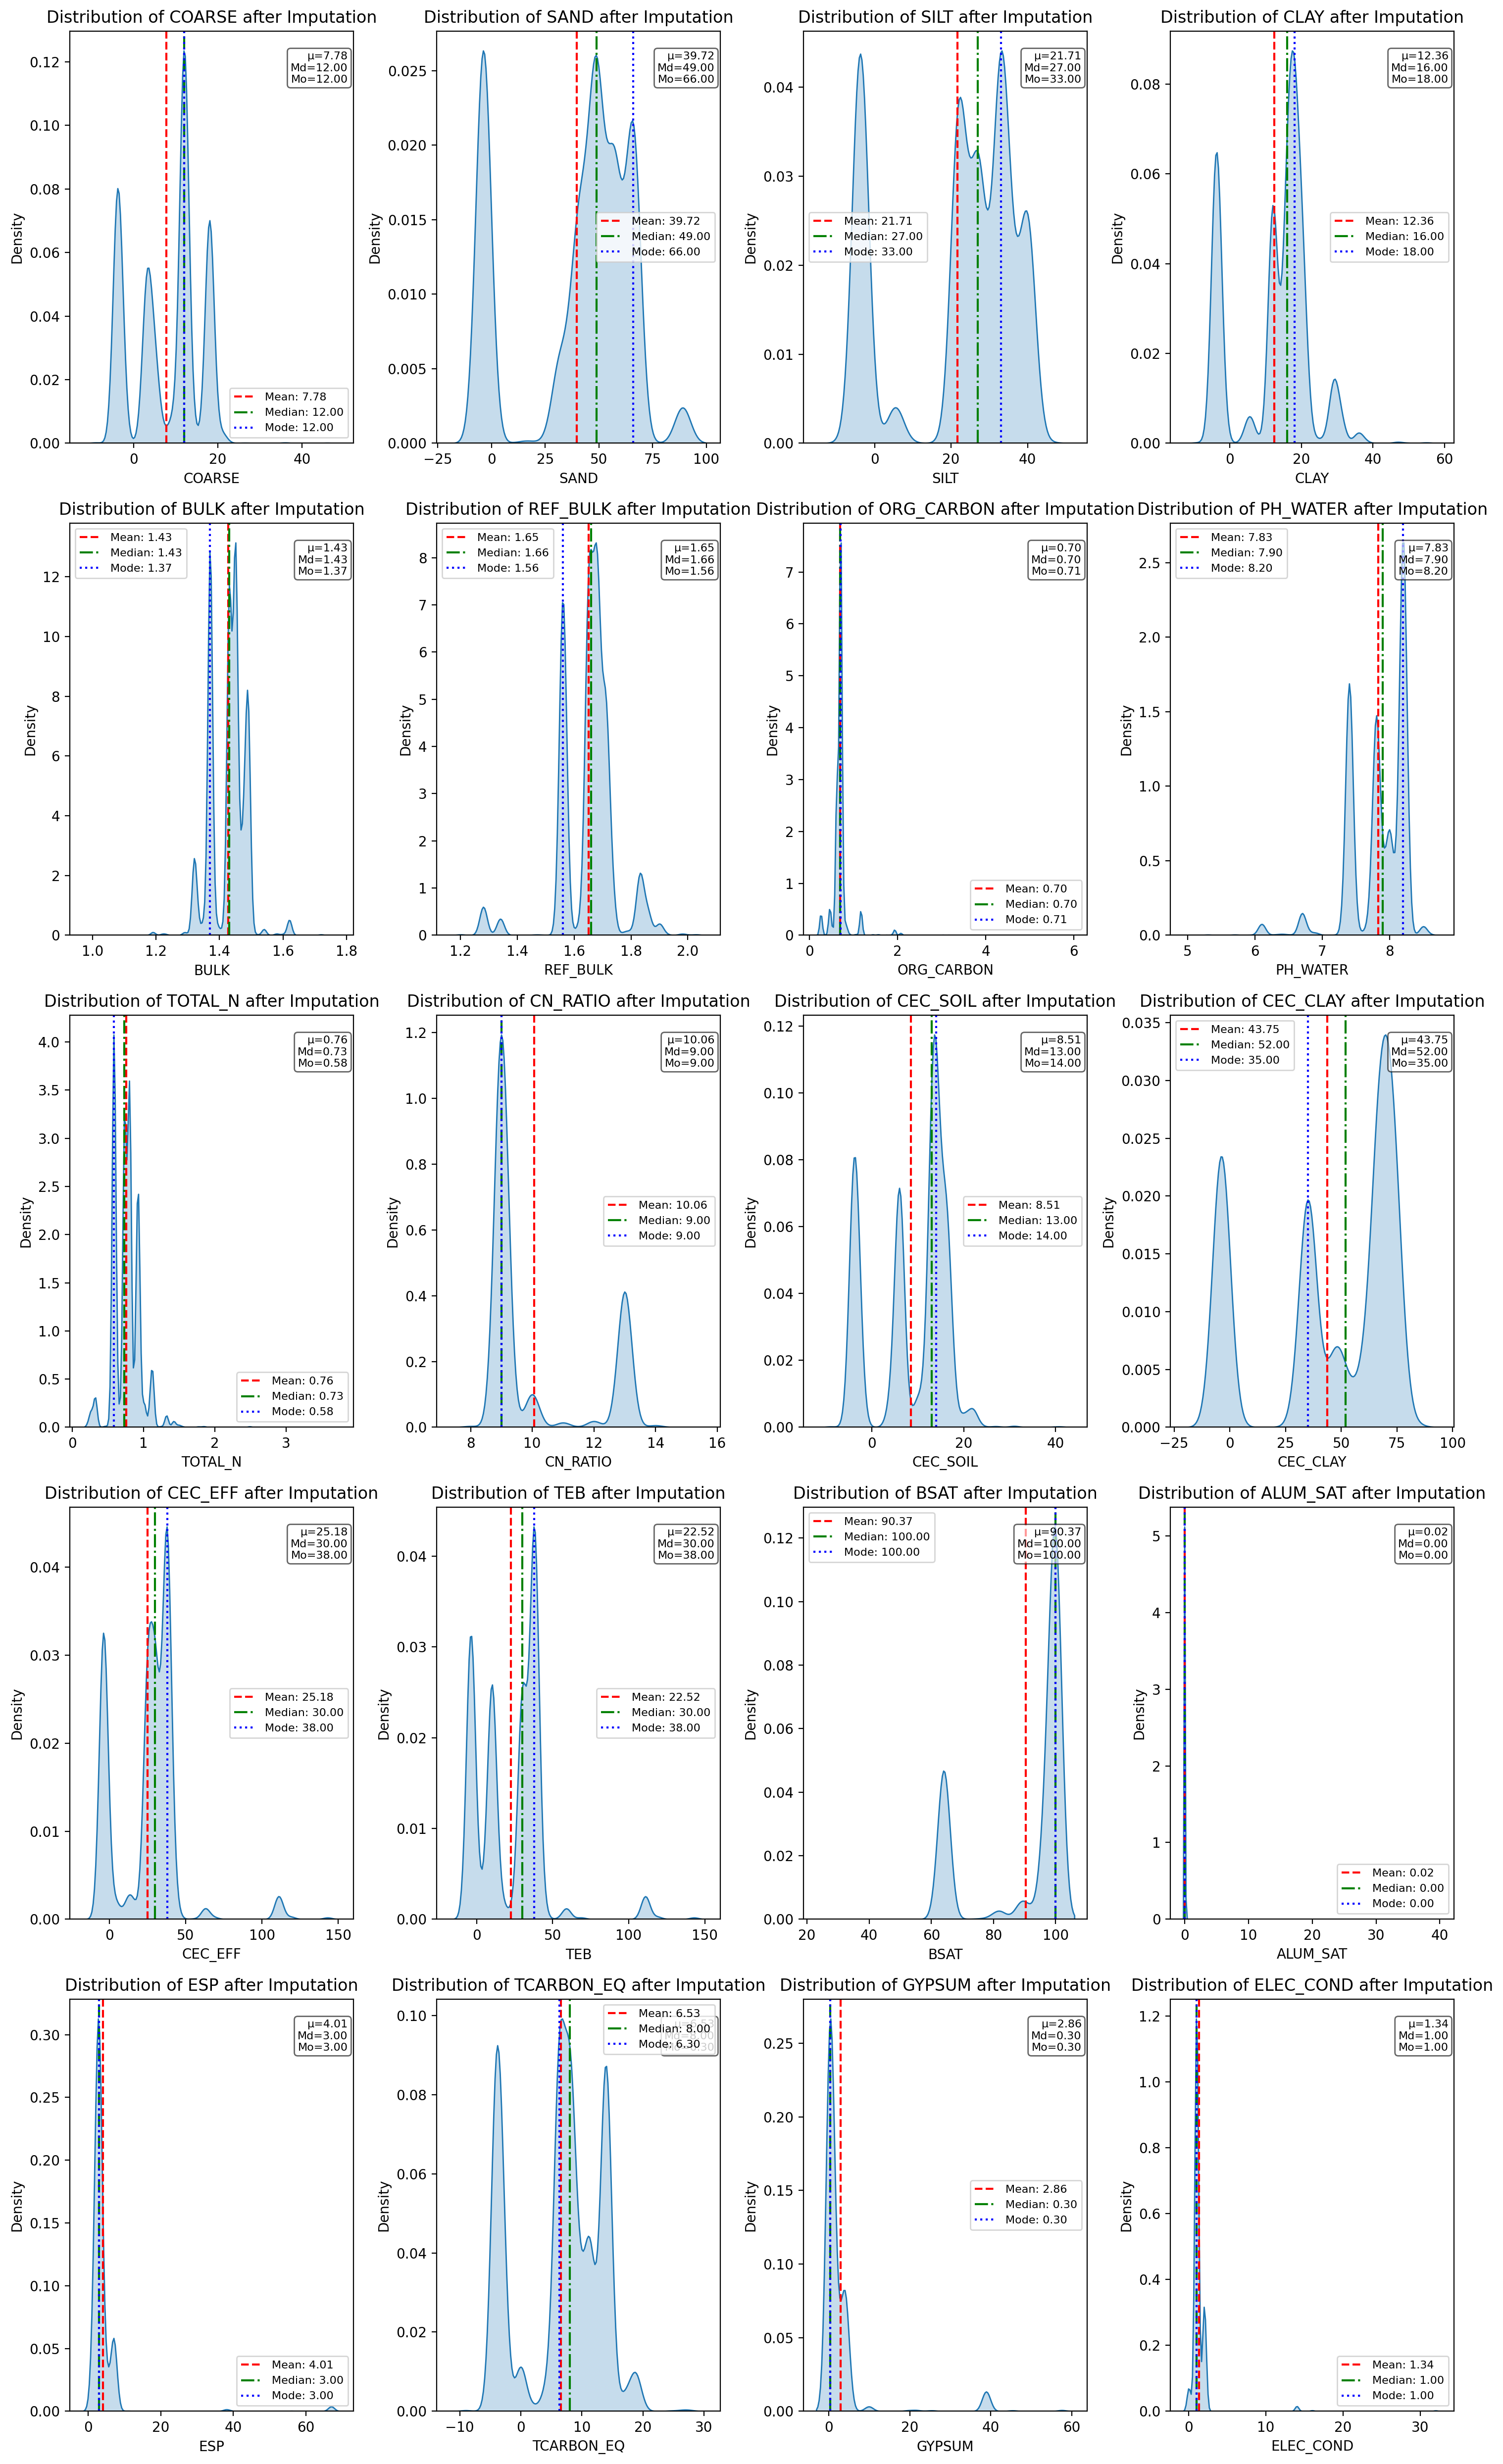
\includegraphics[width=0.65\textwidth]{images/Soil/soil_kde_all_after_imputation.png}
\caption{Kernel density estimates of soil variables after imputation. Vertical lines indicate mean, median, and mode.}\label{fig:soil_kde_after_imputation}
\end{figure}

\begin{figure}[H]
\centering
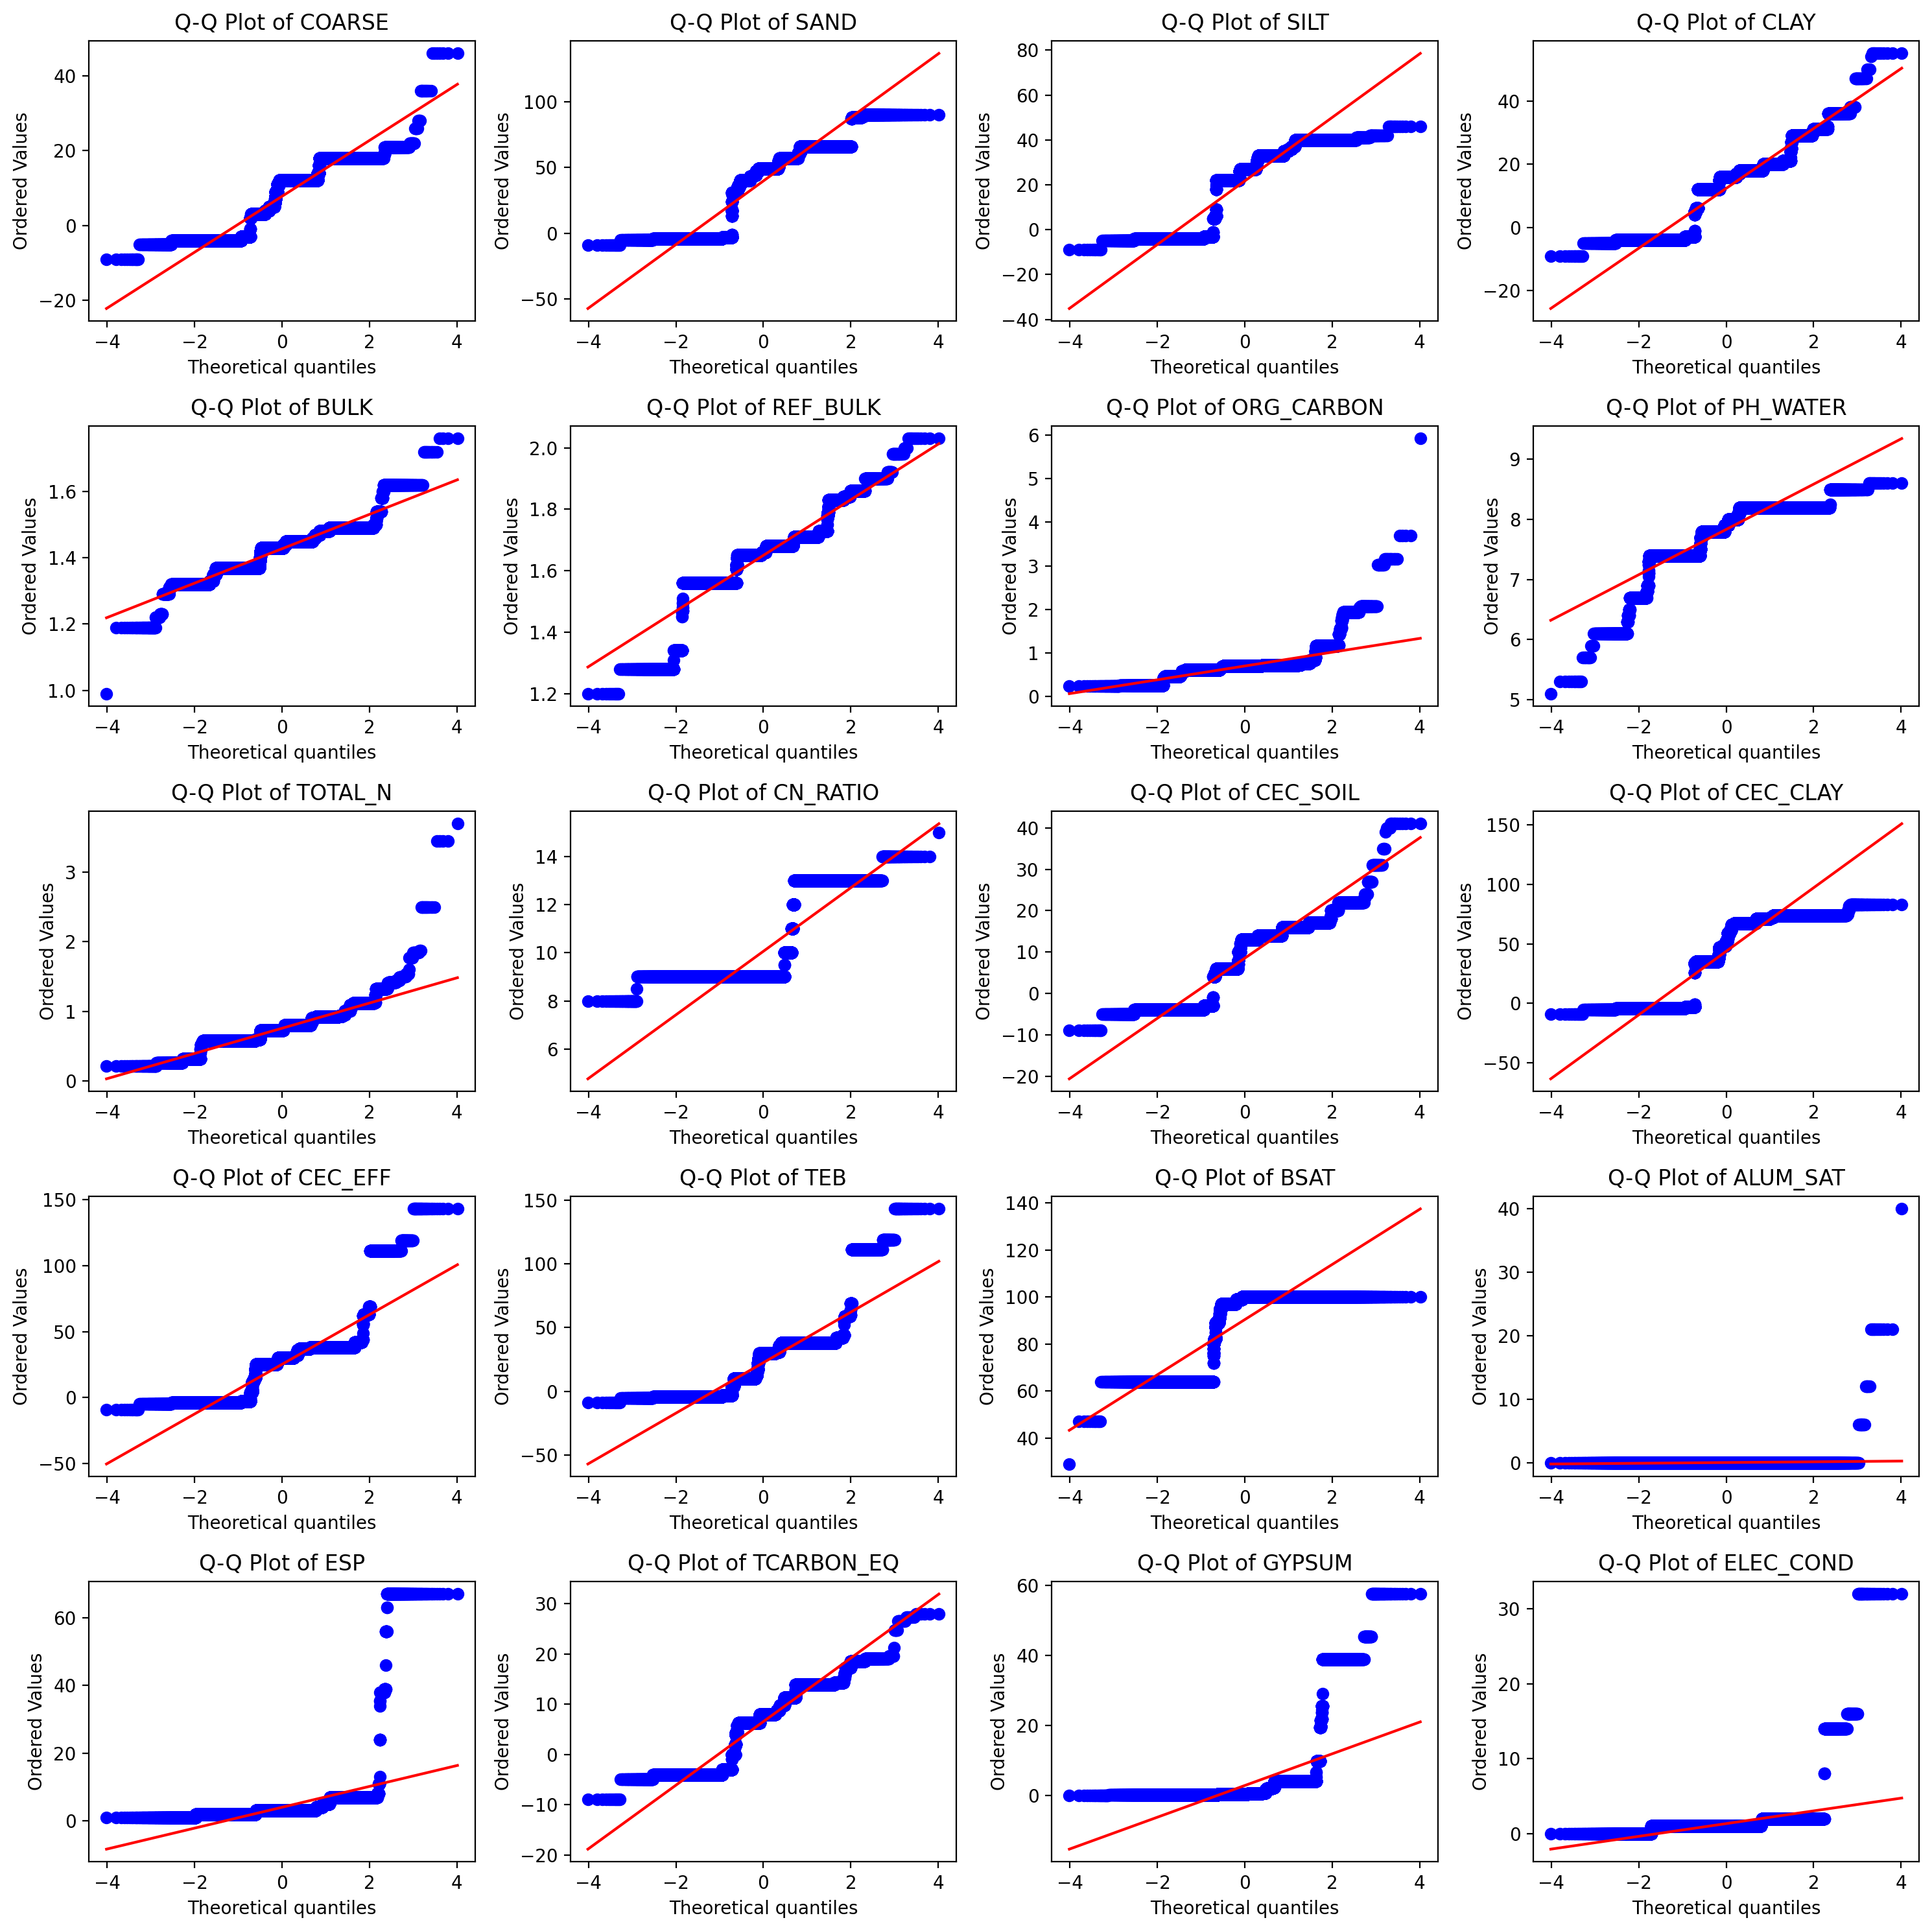
\includegraphics[width=0.65\textwidth]{images/Soil/soil_qq_numeric_after_imputation.png}
\caption{Quantiles plots of numeric soil variables after imputation, highlighting deviations from normality.}\label{fig:soil_qq_after_imputation}
\end{figure}